\chapterimage{slike/Primeri.jpg} 
% Chapter heading image
\chapter{Primeri laserjev}
\label{chap:Primeri}
V tem poglavju bomo spoznali nekaj najpomembnejših vrst laserjev.
V grobem laserje razlikujemo po aktivnem sredstvu 
(plin, trdna snov, organsko barvilo, polprevodnik), pri čemer pa tudi pri izbranem
sredstvu obstaja veliko različnih izvedb in načinov delovanja. Za vsak 
obravnavani primer bomo navedli osnovne karakteristike, v podrobnosti 
izvedbe pa se ne bomo spuščali. 

\section{Laserski sistemi}
\index{Laserski sistemi}
Laser \index{Laser} je lahko dokaj preprosta naprava, z malo sestavnimi deli, 
lahko pa je zelo velik in zapleten sistem. Večina velikih laserskih sistemov
je sestavljena iz osnovnega laserja, ki ni posebno močan, daje pa kvaliteten
snop svetlobe, in iz enega ali več ojačevalnikov. V njih se svetloba 
ojačuje v sredstvu, ki je enako kot v osnovnem laserju in ki je v kolikor 
mogoče visokem stanju obrnjene zasedenosti. V več ojačevalnih korakih 
se tako doseže zelo velika svetlobna moč. 

Pri velikih laserskih močeh nastopi vrsta novih težav. Da gostota 
svetlobnega toka ne povzroča poškodb optičnih komponent, mora 
premer ojačevanega snopa (in s tem premer vseh vmesnih ojačevalnih stopenj) 
naraščati. Zadnje stopnje velikih laserskih sistemov imajo 
tako premer večji od pol metra, kar seveda pomeni, da morajo imeti tolikšno odprtino 
tudi vse ostale optične komponente. Poleg tega je
treba skrbno paziti, da se odbita svetloba ne vrača v prejšnji
ojačevalnik ali v osnovni laser in moti njegovega delovanja. Zato so med
ojačevalnimi stopnjami optični izolatorji, ki temeljijo na Faradayevem
pojavu vrtenja polarizacije v snovi v magnetnem polju.

\begin{figure}[h!]
\centering
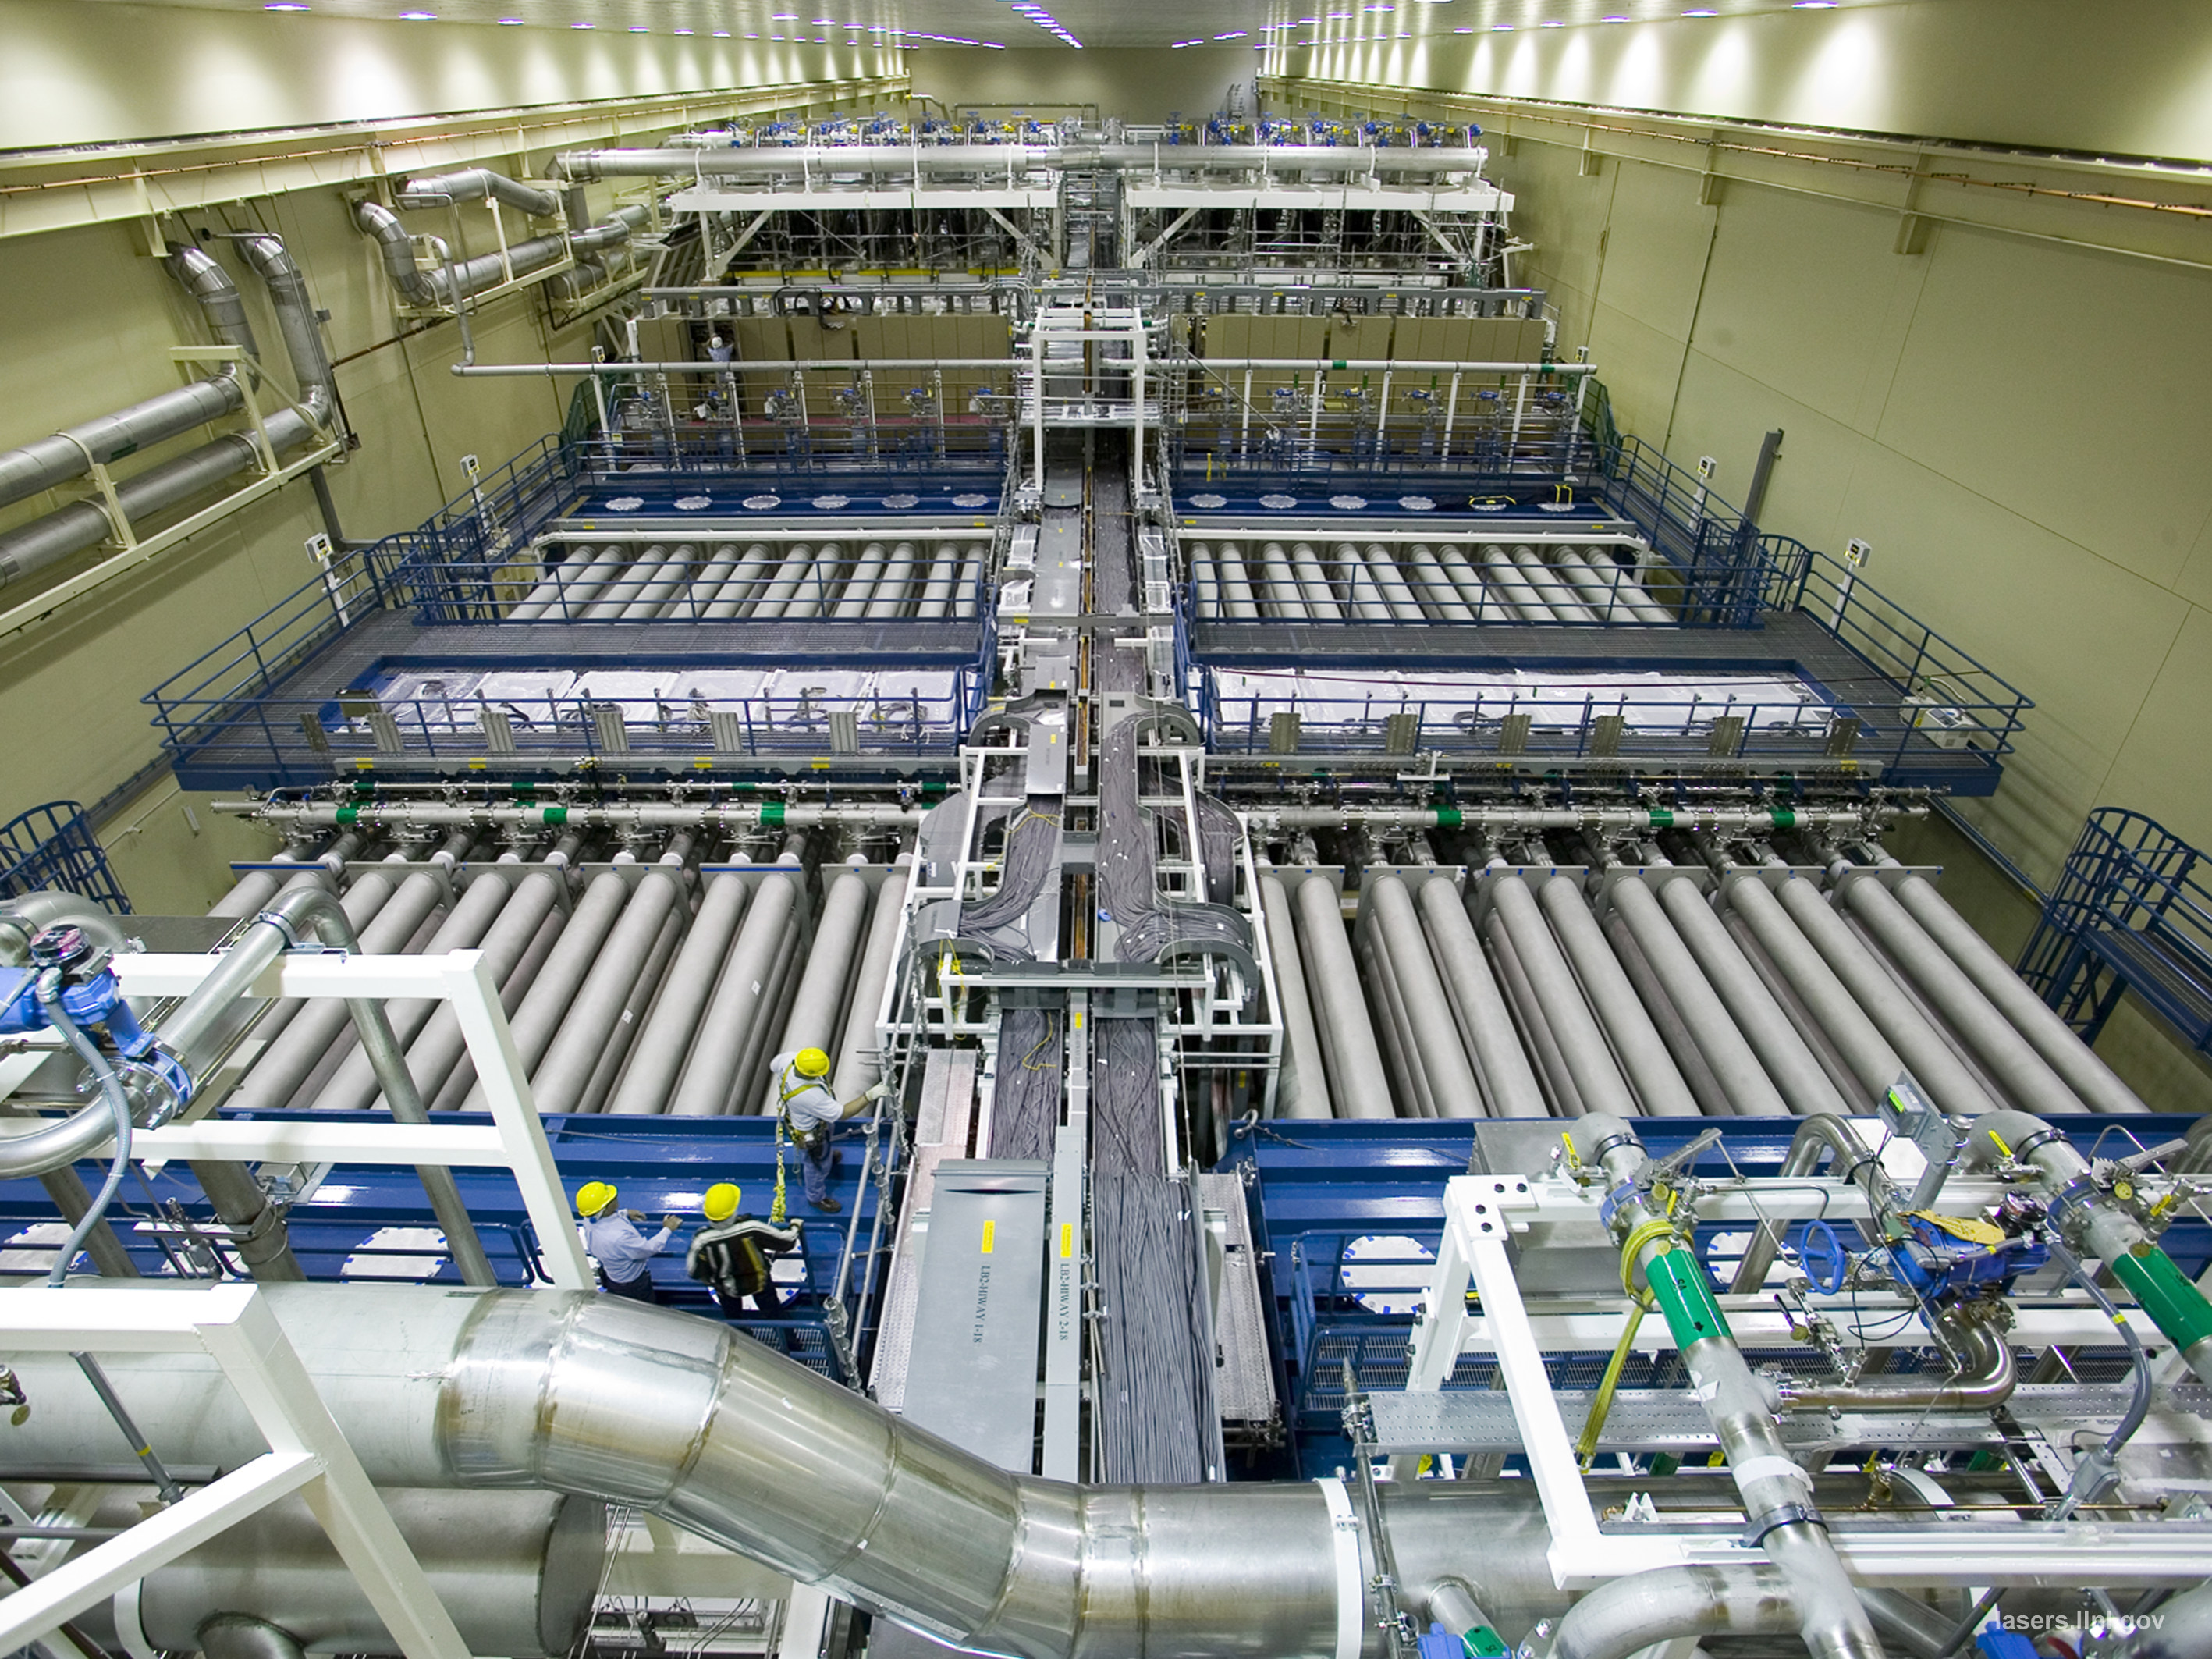
\includegraphics[width=100truemm]{slike/07_NIF_Laser_Bay.jpg}
\caption{Eden najmočnejših laserskih sistemov na svetu, ki doseže 
$500~\si{\tera\watt}$ moči v sunku. \\Vir: National Ignition Facility, Livermore, Kalifornija.}
\label{fig:NIF}
\end{figure}

Moči svetlobe, ki jih oddajajo najmočnejši laserski sistemi, imajo zelo velike
vrednosti. Najmočnejši zvezno delujoči laserji dosegajo tako moči prek 
$\sim 100~\si{\kilo\watt}$. Še bistveno večje moči pa dosegajo sunkovni laserji, 
saj lahko dosežejo moč tudi $\sim 10^{15}~\si{\watt}$. 
Vendar so sunki tako velike svetlobne moči izredno kratki, tipično reda pikosekunde, tako da
znaša celotna moč v takem sunku svetlobe tako ``le'' $\sim \si{\kilo\joule}$. Dodaten 
parameter pri tako močnih sunkovnih laserjih je čas, ki poteče med dvema zaporednima
sunkoma. Najmočnejši laserski sistemi tako lahko izsevajo največ nekaj sunkov dnevno. 

\section{He-Ne laser}
\index{Laser!He-Ne}

Kot prvi primer si oglejmo helij-neon (He-Ne) laser, ki je bil prvi zvezno 
delujoči laser in je še danes zelo razširjen. Najpogosteje deluje 
pri valovni dolžini $632,8~\si{\nano\metre}$ v rdečem delu spektra, poleg 
tega pa tudi pri infrardečih $1,15~\si{\micro\metre}$ in 
$3,39~\si{\micro\metre}$ ter nekaterih drugih
valovnih dolžinah v oranžnem in zelenem delu spektra. Laser deluje v zveznem 
načinu delovanja s tipičnimi močmi $0,5 - 100~\si{\milli\watt}$.

Slika~(\ref{fig:HeNeE}) kaže relevantne energijske nivoje helija in neona. 
\index{Energijski nivoji!He-Ne}
\index{Trinivojski sistem}
Atome helija
s trki z elektroni vzbudimo v eno izmed dveh dolgoživih metastabilnih stanj $2^3S$ ali
$2^1S$ z razpadnima časoma $0,1~\si{\milli\second}$ in $5~\si{\micro\second}$.
Ti dve stanji slučajno praktično sovpadata z dvema stanjema neona ($4s$ in $5s$). 
Ko v helij dodamo razmeroma majhno količino neona, se energija s trki 
prenese z vzbujenih helijevih atomov na atome neona, ki s tem preidejo v 
že omenjeni vzbujeni stanji, helijevi atomi pa se vrnejo v osnovno stanje. 
Majhna energijska razlika med nivoji helija in neona (okoli $1,2~\si{\tera\hertz}$) pri 
tem preide v kinetično energijo obeh atomov. 
\begin{figure}[h]
\centering
\def\svgwidth{100truemm} 
\input{slike/07_HeNeE.pdf_tex}
\caption{Shema energijskih nivojev v He-Ne laserju. Nivoji helija so označeni
z modro in nivoji neona z zeleno, laserski prehodi pa z rdečimi barvami in pripisano
ustrezno valovno dolžino.}
\label{fig:HeNeE}
\end{figure}

Znano rdečo svetlobo He-Ne laserja z valovno dolžino $632,8~\si{\nano\metre}$ dobimo 
pri prehodu iz stanja $5s$ v eno od stanj $3p$. Pri tem je življenjski čas 
stanja $5s$ okoli $100~\si{\nano\second}$, stanja $3p$ pa okoli $10~\si{\nano\second}$.
Spodnji $3p$ nivo se prazni s spontano emisijo v metastabilno stanje $3s$. 
V njem se atomi nabirajo, saj so dipolni sevalni prehodi v osnovno stanje prepovedani,
in atomi le s trki ob steno cevi prehajajo v osnovno stanje. Da pospešimo
praznjenje spodnjega nivoja in povečamo obrnjeno zasedenost, moramo torej 
zmanjšati premer razelektritvene cevi. Zaradi gibanja atomov je spektralna 
črta Dopplerjevo razširjena\index{Dopplerjeva razširitev}. 

Lasersko delovanje dobimo tudi pri prehodu iz $5s$ v stanje $4p$, pri katerem 
ima izsevana svetloba valovno dolžino $3,39~\si{\micro\metre}$. 
Ojačenje je za ta prehod celo precej večje kot za
prehod pri $632,8~\si{\nano\metre}$, deloma zaradi nižje frekvence 
(glej zvezo med Einsteinovima koeficientoma $A$ in $B$, enačba~\ref{4.27}), 
deloma pa zaradi kratke življenjske dobe spodnjega laserskega nivoja $4p$. 
Zato bi pričakovali, da bo He-Ne laser svetil v infrardečem območju in ne vidnem. 
To delno prepreči absorpcija v steklu, delno pa izgube namerno povečamo s selektivno odbojnostjo
resonatorskih zrcal, ki dvigne prag delovanja za $3,39~\si{\micro\metre}$ 
nad prag za $632,8~\si{\nano\metre}$. V nekaterih primerih v laser dodamo
celico metana, ki infrardečo svetlobo močno absorbira, rdeče pa ne.
Omenimo še prehode iz stanja $4s$, ki ga dosežejo neonovi atomi s trki
z vzbujenimi helijevimi atomi iz nivoja $2^3S$. Prehod $4s$ v $3p$, ki da svetlobo
pri $1,15~\si{\micro\metre}$, je bil prvi opaženi prehod v He-Ne laserjih.

Tipičen He-Ne laser je razmeroma preprosto zgrajen (sliki~\ref{fig:HeNeShema}
in \ref{fig:Iskra}).\index{Laser!zgradba}
V razelektritveni cevi (napetost  $\sim 1~\si{\kilo\volt}$), skozi
katero teče električni tok ($\sim 10~\si{\milli\ampere}$), 
se nahaja mešanica helija in neona v razmerju 
$5:1 - 10:1$. Skupni tlak v cevi je nizek, le okoli $3~\si{\milli\bar}$, 
cev pa je tipično dolga okoli $0,5~\si{\metre}$ s premerom $1-2~\si{\milli\metre}$.  
Cev na obeh straneh zapirata okni, ki sta nagnjeni za Brewstrov kot (glej enačbo~\ref{eq:Brew}), 
tako da so izgube pri odboju za eno polarizacijo kar se da majhne.
Izhodna svetloba iz laserja je zato seveda polarizirana. V manjših laserjih
so namesto Brewstrovih oken na razelektritveno cev privarjena kar
resonatorska zrcala. Tak laser je nepolariziran. 
Razelektritvena cev je obdana z dvema ukrivljenima zrcaloma, 
ki imata zelo veliko odbojnost za izbrano valovno dolžino.
Nekaj tipičnih podatkov za He-Ne laser je zbranih v tabeli~(\ref{tab:Ar}).
\begin{figure}[h]
\centering
\def\svgwidth{100truemm} 
\input{slike/07_HeNeShema.pdf_tex}
\caption{Shema He-Ne laserja: R - razelektritvena cev, IZ - izhodno zrcalo, Z - zrcalo
z veliko odbojnostjo, B - Brewstrovi okni}
\label{fig:HeNeShema}
\end{figure}

\begin{figure}[h]
\centering
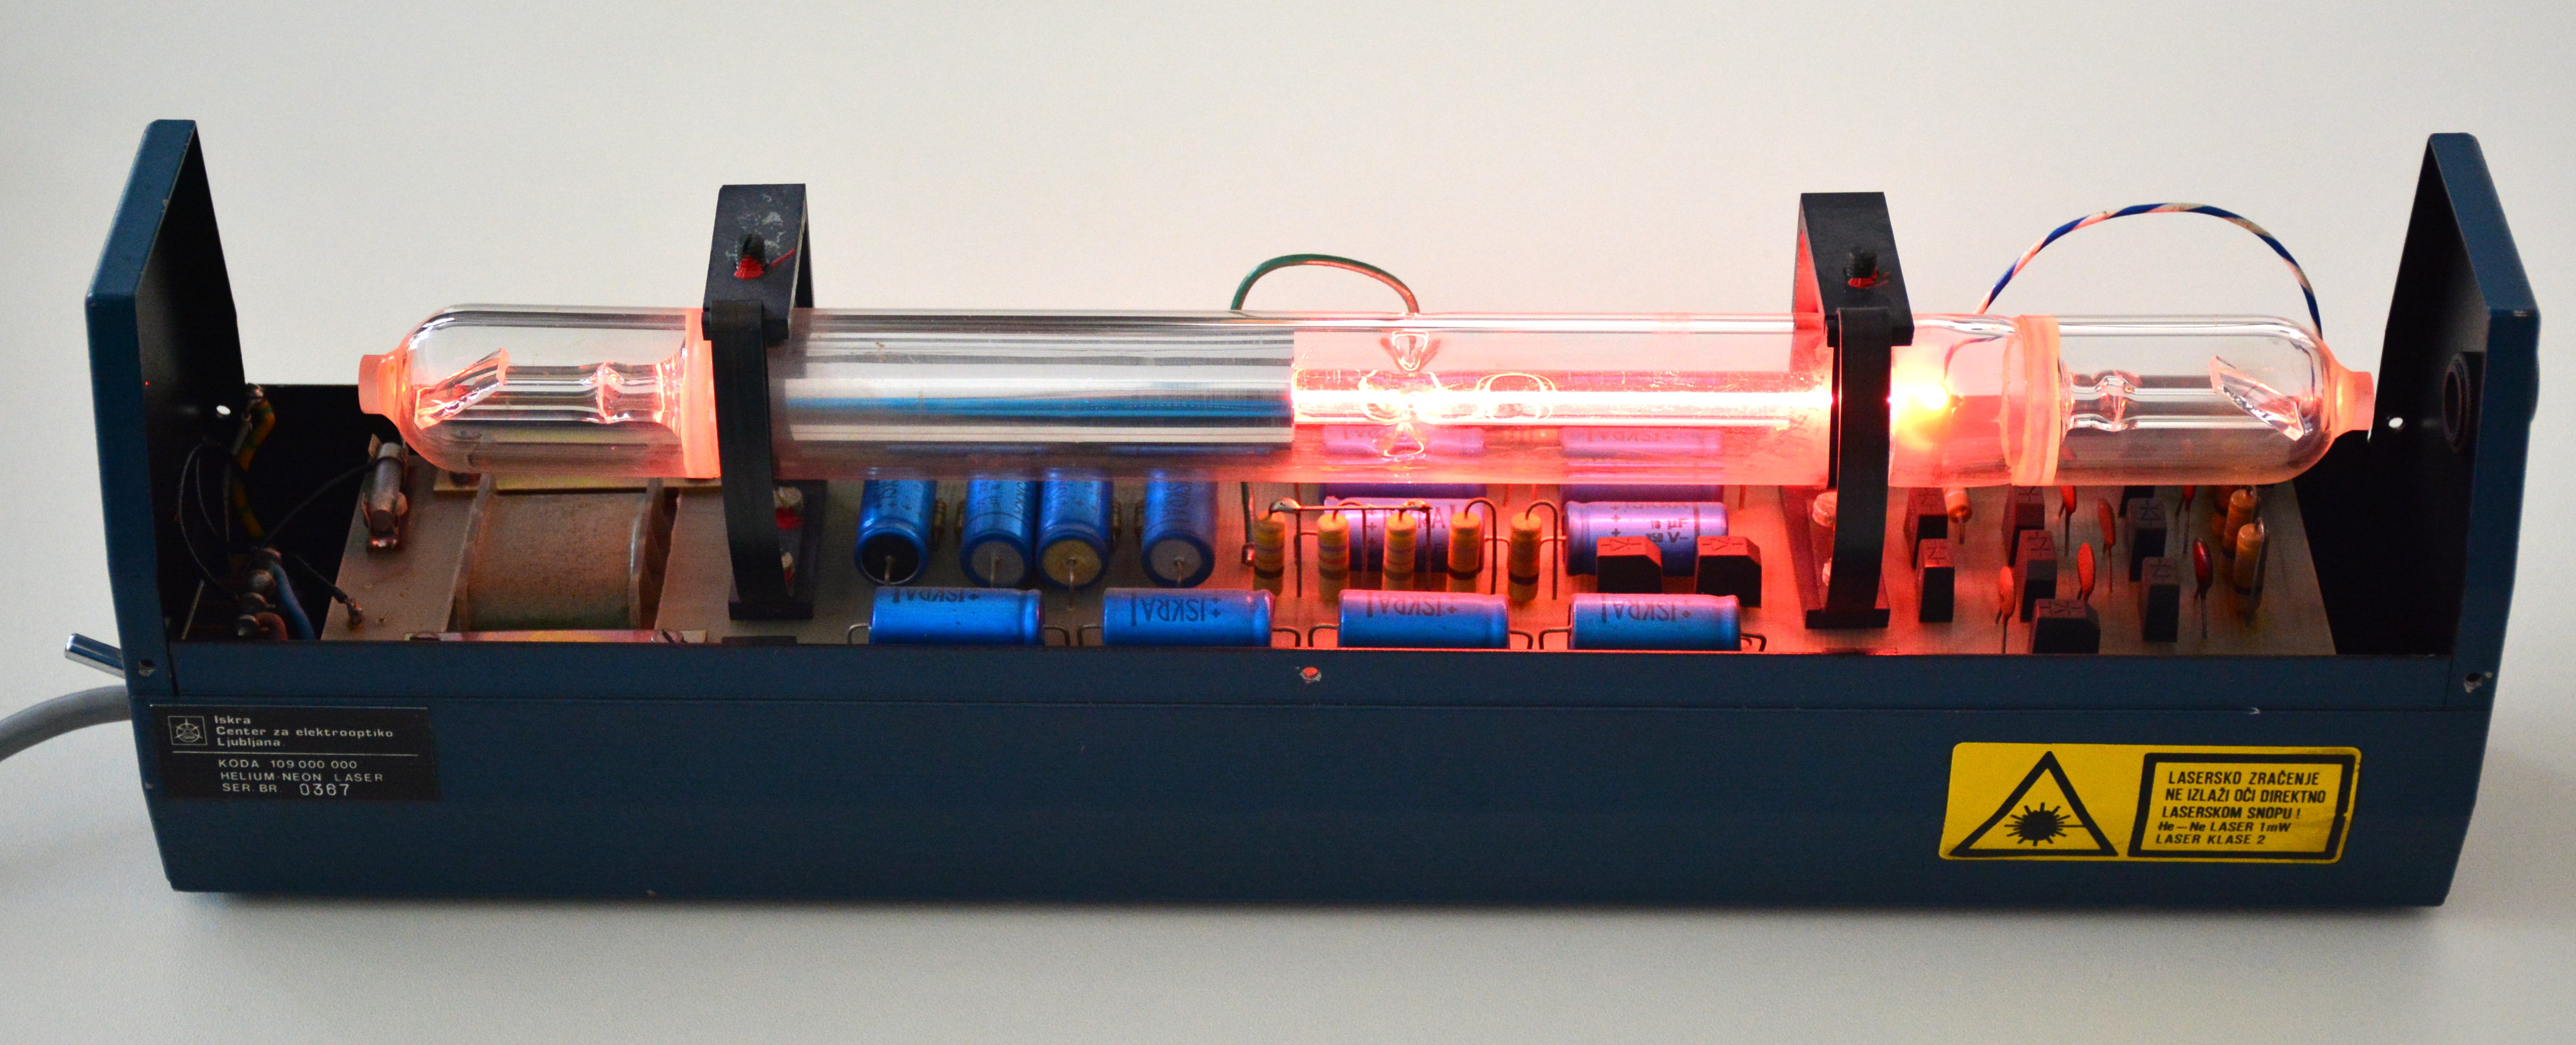
\includegraphics[width=120truemm]{slike/07_HeNe.jpg}
\caption{Primer starejšega He-Ne laserja, izdelanega v Sloveniji}
\label{fig:Iskra}
\end{figure}

He-Ne laserji so preprosti, stabilni, zanesljivi, poceni, imajo visoko kvaliteto žarka
in dolgo služijo (do 50 000 ur).
Danes jih sicer izrivajo polprevodniški laserji, vendar so še vedno v uporabi
v merilnih napravah, v optičnih čitalnih sistemih, v šolah, v raziskovalnih 
laboratorijih za interferometrijo, holografijo itd. Na njem je osnovan tudi 
sekundarni standard za meter.

\section{Argonski ionski laser}
\index{Laser!argonski}
\index{Štirinivojski sistem}
Kot drugi primer plinskega laserja obravnavajmo argonski ionski (Ar$^+$) laser,
ki je najbolj poznan po zveznem delovanju v modrem in zelenem delu spektra pri 
valovnih dolžinah $488~\si{\nano\metre}$ in $514,4~\si{\nano\metre}$, deluje 
pa tudi v bližnjem ultravijoličnem območju. Tipične moči delovanja argonskega laserja
so $100~\si{\milli\watt} - 50~\si{\watt}$.

Kot večino drugih plinskih laserjev tudi tega črpamo z električnim tokom.
Atome argona vzbudimo s trki z elektroni v ione argona, ti pa z nadaljnjimi
trki preidejo v vzbujena stanja. Obrnjeno zasedenost
dosežemo med nivojema $4p$ in $4s$ (slika~\ref{fig:ArE}). 
Ta dva nivoja vsebujeta veliko podnivojev, zato je tudi prehodov med
njima zelo veliko. Argonski laser tako seva pri več kot tridesetih različnih
valovnih dolžinah, najznačilnejši sta že omenjeni 488~nm in 514,5~nm. 
Življenjski čas zgornjega nivoja $\sim 10^{-8}~\si{\second}$ je približno 
desetkrat daljši od življenjskega časa spodnjega nivoja, od koder se ioni
z rekombinacijo z elektroni vrnejo v osnovno stanje atoma. Tudi pri tem laserju
je poglavitni vzrok za razširitev črte \index{Dopplerjeva razširitev}Dopplerjev 
pojav.\index{Energijski nivoji!argon}

\begin{figure}[h]
\centering
\def\svgwidth{80truemm} 
\input{slike/07_ArE.pdf_tex}
\caption{Shema energijskih nivojev v Ar$^+$ laserju}
\label{fig:ArE}
\end{figure}

Argonski laser je v osnovi zgrajen podobno kot He-Ne laser. \index{Laser!zgradba}
V razelektritveni cevi
(tipična dolžina $1~\si{\metre}$ in premer $1-2~\si{\milli\metre}$)
se nahaja argon pri pritisku okoli $10~\si{\milli\bar}$. Ker gre pri 
vzbujanju atomov argona za dvostopenjski proces, mora biti električni tok, 
s katerim dosežemo obrnjeno zasedenost, precej velik, lahko tudi nekaj deset amperov. 
Pri tipični napetosti nekaj kV to pomeni, da so potrebne velike električne moči, 
pogosto več deset $\si{\kilo\watt}$, in močnejši argonski laserji so zato zaradi 
velike količine odvečne toplote najpogosteje vodno hlajeni.

\begin{figure}[h]
\centering
\def\svgwidth{110truemm} 
\input{slike/07_ArShema.pdf_tex}
\caption{Poenostavljena shema Ar laserja s prizmo: R - razelektritvena cev, 
IZ - izhodno zrcalo, Z - zrcalo z veliko odbojnostjo, B - Brewstrovi okni, 
P - prizma
}
\label{fig:ArS}
\end{figure}

V argonskih laserjih pogosto ustvarimo tudi vzdolžno magnetno polje, ki preprečuje 
elektronom, da bi predčasno zapustili ojačevalno območje in trčili v steno. S
tem se poveča izhodna moč laserja, hkrati pa preprečuje poškodbe na stenah, ki bi jih 
lahko povzročili visokoenergijski elektroni. Iz istega razloga so pri močnejših
laserjih zrcala izven plinske cevi. 

V resonator argonskega laserja pa moramo vgraditi še en dodaten element, ki omogoči
izbiro ene same spektralne črte. Najpogosteje za ta frekvenčno selektiven element
uporabimo kar majhno prizmo pred enim od obeh zrcal (slika~\ref{fig:ArS}). Zaradi disperzije
v prizmi se snopi različnih valovnih dolžin lomijo pod različnimi koti in le tisti 
snop, ki vpada pravokotno na zrcalo, je ojačan. Z vrtenjem prizme ali zrcala lahko 
tako izberemo valovno dolžino ojačene svetlobe. Nekaj tipičnih podatkov za argonski
laser je zbranih v tabeli~(\ref{tab:Ar}).

Argonski laser je zanesljiv in daje zelo kvaliteten osnovni Gaussov snop pri eni
sami frekvenci. Zato se dosti uporablja v optični spektroskopiji,
interferometriji, holografiji in merilni tehniki. Deluje lahko v zveznem načinu,
zaradi razmeroma široke črte ojačenja pa ga uporabljamo tudi za fazno uklenjen
sunkovni laser z dolžino sunkov okoli $150~\si{\pico\second}$. 
V kombinaciji s kriptonovim laserjem, ki je zelo podoben argonskemu, le da deluje
v rdečem in oranžnem delu spektra, se uporablja tudi v zabavni industriji.
V zadnjem času ga vse bolj izrivajo polprevodniški laserji ali pa frekvenčno
podvojeni Nd:YAG. 

\section{Laser na ogljikov dioksid}
\index{Laser!CO$_2$}
Do zdaj opisani laserji so delovali na elektronskih prehodih v atomih oziroma ionih. 
Laser na ogljikov dioksid pa deluje na prehode med vibracijskimi stanji molekul 
CO$_2$, pri čemer elektroni ostanejo v osnovnem stanju.
Zaradi majhnih energijskih razlik med vibracijskimi stanji deluje
tak laser v infrardečem delu spektra, najpogosteje pri 
$9,6~\si{\micro\metre}$ in $10,6~\si{\micro\metre}$. Laser deluje v zveznem
in v sunkovnem načinu, odlikuje ga pa zelo velik izkoristek ($~\sim 30~\%$) in 
posledično zelo velike moči, $1~\si{\watt} - 10~\si{\kilo\watt}$. 

Preden opišemo delovanje laserja, si na kratko oglejmo še nihajna stanja molekule 
ogljikovega dioksida. Molekula CO$_2$ je v osnovnem stanju linearna molekula 
(slika~\ref{fig:CO2}\,a). 
Za molekule take oblike obstajajo trije osnovni načini nihanja atomov glede na težišče:
atoma kisika nihata simetrično vzdolž osi molekule, pri čemer ogljik miruje --
simetrični razteg (slika~\ref{fig:CO2}\,b), atomi nihajo v smeri pravokotno na 
os -- upogib (slika~\ref{fig:CO2}\,c) in atoma kisika se gibljeta v isti smeri 
vzdolž osi, ogljik pa v nasprotni smeri -- asimetrični razteg (slika~\ref{fig:CO2}\,d). 
Pri tem ima najvišjo frekvenco asimetrični razteg, najnižjo pa upogib. 
Vsako vibracijsko stanje lahko razstavimo na osnovne nihajne načine in 
ga opišemo s številom energijskih kvantov v posameznem osnovnem nihanju, 
torej s trojico celih števil $(n_1,n_2,n_3)$. Stanje 100 tako opisuje
osnovni simetrični razteg, stanje 010 osnovno upogibno nihanje, stanje 001 pa 
osnovni asimetrični razteg.

\begin{figure}[h]
\centering
\def\svgwidth{100truemm} 
\input{slike/07_CO2.pdf_tex}
\caption{Molekula CO$_2$ (a) in trije osnovni načini nihanja molekule:
simetrični razteg (b), upogib (c) in asimetrični razteg (d)}
\label{fig:CO2}
\end{figure}

Vibracijska stanja molekule vzbudimo z električnim tokom skozi plin. 
\index{Energijski nivoji!CO$_2$}
\index{Štirinivojski sistem}
Pri tem v razelektritveno cev dodamo dušik (N$_2$) in podobno kot pri He-Ne laserju
se tudi CO$_2$ črpa predvsem preko trkov z dušikovimi molekulami. 
Dušikova molekula je dvoatomna in ima zato zgolj eno vibracijsko stanje, ki po energiji
praktično sovpada z energijo stanja 001 (slika~\ref{fig:CO2E}). Iz tega gornjega
stanja prehajajo molekule v stanje 100 ($10,6~\si{\micro\metre}$) ali v stanje
020 ($9,6~\si{\micro\metre}$). Da pospešimo prehod nazaj v osnovno stanje, 
plinski mešanici dodamo še helij, s katerim trkajo molekule.
Razmerje parcialnih tlakov je tako navadno 1:1:8 za CO$_2$:N$_2$:He pri tlaku $1~\si{\milli\bar}$. 
Pri tako nizkih tlakih je poglavitna razširitev spektralne črte Dopplerjeva, 
\index{Dopplerjeva razširitev}ki 
pa je v primerjavi z ostalimi plinskimi laserji zaradi nizih frekvenc zelo majhna,
le okoli $70~\si{\mega\hertz}$. V laserskih sistemih, kjer je tlak plinov večji,
prevlada razširitev zaradi medmolekulskih trkov. Pri tlakih okoli $20~\si{\bar}$
znaša razširitev že okoli $500~\si{\giga\hertz}$, kar omogoča izdelavo fazno uklenjenih 
sunkovnih laserjev s sunki dolžine $\sim 1~\si{\pico\second}$. Nekaj tipičnih podatkov 
za laser na ogljikov dioksid je zbranih v tabeli~(\ref{tab:Ar}).

\begin{figure}[h]
\centering
\def\svgwidth{95truemm} 
\input{slike/07_CO2E.pdf_tex}
\caption{Shema vibracijskih nivojev v CO$_2$ laserju}
\label{fig:CO2E}
\end{figure}

Najpreprostejši laser na ogljikov dioksid \index{Laser!zgradba} 
je po svoji zgradbi podoben že obravnavanim plinskim laserjem. 
Razelektritvena cev (polmer $\sim 1~\si{\centi\metre}$ in dolžina $0,5-2~\si{\metre}$) 
je na obeh koncih zaključena z Brewstrovima oknoma in zrcaloma, pri čemer moramo paziti,
da elementi prepuščajo oziroma odbijajo infrardečo svetlobo. Ker lahko deluje
laser pri zelo veliko različnih valovnih dolžinah, dodamo frekvenčno selektiven
člen, na primer uklonsko mrežico (slika~\ref{fig:CO2S}).\index{Uklonska mrežica}

\begin{figure}[h]
\centering
\def\svgwidth{100truemm} 
\input{slike/07_CO2Shema.pdf_tex}
\caption{Poenostavljena shema najpreprostejšega CO$_2$ laserja: R - razelektritvena cev, 
IZ - izhodno zrcalo, Z - zrcalo z veliko odbojnostjo, B - Brewstrovi okni, 
U - uklonska mrežica
}
\label{fig:CO2S}
\end{figure}

Poleg običajnih zaprtih sistemov poznamo tudi laserje z vzdolžnim ali prečnim pretokom, 
valovodne laserje ... Razlikujejo se po svojih specifikacijah in vrsti uporabe.
Laserji na ogljikov dioksid se največ uporabljajo v industriji za zahtevne 
obdelave materialov, na primer za rezanje 
kovin, vrtanje, ablacijo, varjenje, pa tudi za vojaške in medicinske namene.
Obdelava z laserji omogoča veliko natančnost, čistočo in je zelo fleksibilna.

\begin{table}
\small
\begin{center}
\begin{tabular}{|l|c|c|c|c|}\hline
Laser & He-Ne & Ar$^+$ & CO$_2$ & ekscimer\\ \hline
Valovna dolžina  $\lambda$ & $632,8~\si{\nano\metre}$& $488$ in
$514,5~\si{\nano\metre}$ & $9,6$ in $10,6~\si{\micro\metre}$ & UV
\\ \hline
Verjetnost za spontani prehod $A$ & $3,4 \times 10^6/\si{\second}$ & 
$7,8 \times 10^7/\si{\second}$ & $0,25/\si{\second}$ & $\sim 10^8/\si{\second}$ \\ \hline
Presek za stimulirano emisijo $\sigma$ & $3 \times 10^{-17}~\si{\metre}^2$&  $2,6 \times 10^{-16}~\si{\metre}^2$ & $3 \times 10^{-22}~\si{\metre}^2$ & $ 10^{-20}~\si{\metre}^2$ \\ \hline
Spektralna širina črte $\Delta \nu$ & $1,5 \times 10^{9}~\si{\hertz}$ & 
$3,5 \times 10^{9}~\si{\hertz}$ &$7 \times 10^{7}~\si{\hertz}$ & $10^{13}~\si{\hertz}$ \\ \hline
Obrnjena zasedenost $\Delta N/V$ & $5 \times 10^{15}/\si{\metre}^3$ & $2 \times 10^{15}/\si{\metre}^3$ & $3 \times 10^{21}/\si{\metre}^3$ & $10^{20}/\si{\metre}^3$\\ \hline
\end{tabular}
\caption{Izbrani podatki za He-Ne, Ar$^+$, CO$_2$ in tipičen ekscimerni laser}
\index{Laser!He-Ne}
\index{Laser!argonski}
\index{Laser!CO$_2$}
\index{Laser!ekscimerni}
\label{tab:Ar}
\end{center}
\end{table}

\section{Ekscimerni laser}
\index{Laser!ekscimerni}
Ekscimerji ({\it excited dimer, excimer}) so vzbujena vezana stanja dveh atomov, 
ki bi se v osnovnem stanju ne vezala. Za laserje so zanimivi predvsem ekscimerji
težkih žlahtnih plinov in halogenov, na primer Ar$_2^*$ ($126~\si{\nano\metre}$), 
Kr$_2^*$ ($146~\si{\nano\metre}$), Xe$_2^*$ ($172~\si{\nano\metre}$),
ArF ($193~\si{\nano\metre}$), KrF ($248~\si{\nano\metre}$), 
XeCl ($308~\si{\nano\metre}$), ArBr ($161~\si{\nano\metre}$), 
NeF ($108~\si{\nano\metre}$) ... Te molekule obstajajo samo v vzbujenem stanju,
v osnovnem stanju pa je odbojna sila med atomoma prevelika in molekula neobstojna.
Vsi našteti primeri oddajajo lasersko svetlobo v
ultravijoličnem področju, ki ga drugi laserski sistemi le težko pokrivajo. 
Ekscimerni laserji delujejo v sunkih, pri čemer je tipična oddana energija v sunku 
$\sim 1~\si{\joule}$, dolžina sunka $10-100~\si{\nano\second}$ in repeticija 
$\sim 100~\si{\hertz}$.

Vezano stanje dveh atomov dobimo, kadar je ionizacijska energija prvega
atoma manjša od vsote elektronske afinitete drugega atoma in
elektrostatične energije vezave obeh ionov. Vzemimo za primer klor in
kripton. Ionizacijska energija kriptona v osnovnem stanju je 14~eV, v
vzbujenem pa 5~eV. Elektronska afiniteta klora je 3,75~eV in
elektrostatična vezavna energija KrCl okoli 7~eV. Tako je za nastanek
molekule KrCl v osnovnem stanju potrebno dodati okoli 4~eV, pri tvorbi
molekule v vzbujenem stanju pa se sprosti okoli 6~eV. Približno obliko
celotne potencialne energije molekule KrCl v osnovnem in vzbujenem stanju
kaže slika~(\ref{fig:exE}). Molekula, ki je vezana v vzbujenem stanju, po
sevalnem prehodu v osnovno stanje takoj razpade, zato je zelo lahko doseči
obrnjeno zasedenost. Pri tem je razpadni čas vezanega stanja $\sim~10~\si{\nano\second}$,
spodnjega nevezanega pa okoli $0,1~\si{\pico\second}$.
Spektralna širina prehoda je precej velika, okoli $1~\si{\nano\metre}$.
Da nastanejo ekscimeri, vzbujamo mešanico 
plinov (žlahtnega plina ali mešanice žlahtnega in halogenega plina) v heliju. Ker je pritisk
razmeroma velik (npr. 2 ali $3~\si{\bar}$), je vzbujanje prečno, podobno kot pri 
nekaterih izvedbah CO$_2$ laserja. Nekaj tipičnih podatkov 
za ekscimerni laser je zbranih v tabeli~(\ref{tab:Ar}).
\index{Energijski nivoji!ekscimer}

Ekscimerni laserji delujejo v sunkih s precej veliko energijo in se uporabljajo 
v industriji materialov, mikroprocesorjev, fotolitografiji in medicini, predvsem 
oftalmologiji in kirurgiji.
\begin{figure}[h]
\centering
\def\svgwidth{50truemm} 
\input{slike/07_exE.pdf_tex}
\caption{Shema energije v odvisnosti od razdalje med jedroma atomov. V vzbujenem stanju
se atoma povežeta v molekulo, po prehodu v nižji nivo pa atoma disociirata.}
\label{fig:exE}
\end{figure}


\section{Neodimov laser}
Druga skupina laserjev so trdninski laserji. Taki laserji
so osnovani na elektronskih prehodih v ionih primesi, ki jih dodamo v kristal ali steklo,
črpamo pa jih optično. Primesi so praviloma redke zemlje ali prehodne kovine, 
kristali pa so navadno oksidi ali fluoridi. Izdelava ojačevalnih sredstev na osnovi stekla
je bistveno bolj preprosta in poceni, vendar ima steklo precej nižjo toplotno prevodnost
od kristalov in se zato bolj greje. 
Začeli bomo z opisom dveh primerov neodimovega laserja, Nd:YAG in Nd:steklo. Podobne laserje dobimo, 
če v YAG kristalu namesto z neodimom itrijeve ione nadomestimo z iterbijem ($1030~\si{\nano\metre}$) ali erbijem ($2940~\si{\nano\metre}$).

\subsection{Nd:YAG}
\index{Laser!Nd:YAG}
Najpomembnejši predstavnik je Nd:YAG laser, v katerem je ojačevalno sredstvo
itrij-aluminijev granat (Y$_3$Al$_5$O$_{12}$, YAG) s primesmi neodimovih ionov Nd$^{3+}$. 
Neodimov laser deluje pri valovni dolžini $1,064~\si{\micro\meter}$ ali frekvenčno podvojeni
$532~\si{\nano\metre}$. Laser lahko deluje v zveznem 
načinu pri močeh $5-100~\si{\watt}$ ali sunkovnem z dolžino sunkov okoli 
$100~\si{\nano\second}$ in energijo sunka $\sim 1~\si{\joule}$.

Neodimov laser je primer štirinivojskega laserskega sistema, 
\index{Štirinivojski sistem}pri čemer je 
laserski prehod med stanjema $^4$F$_{3/2}$ in $^4$I$_{11/2}$ iona neodima 
(slika~\ref{fig:NdE}). S svetlobo višje frekvence 
(tipično okoli $800~\si{\nano\metre}$) črpamo elektrone v višje nivoje, ki hitro 
preidejo v zgornji laserski nivo. Življenjski čas višjega nivoja je 
okoli $230~\si{\micro\second}$, spodnjega pa precej krajši, zato je 
lahko doseči veliko obrnjeno zasedenost. Spodnje stanje je dovolj visoko nad 
osnovnim, da pri sobni temperaturi v ravnovesju ni znatno zasedeno. Zato je 
prag neodimovega laserja nizek in je lahko doseči zvezno stacionarno delovanje, 
prav tako dobro pa deluje tudi v sunkih. Razširitev črte je homogena in je predvsem posledica
termičnega nihanja kristalne mreže. Laser je odličen za delovanje s preklopom dobrote, 
zaradi ozke črte pa z uklepanjem faz oddaja zelo kratke sunke (nekaj ps). 
\index{Energijski nivoji!Nd:YAG}
\begin{figure}[h]
\centering
\def\svgwidth{85truemm} 
\input{slike/07_NdE.pdf_tex}
\caption{Shema energijskih nivojev v Nd$^{3+}$ laserju}
\label{fig:NdE}
\end{figure}

Za črpanje uporabljamo diodne laserje ali močne ksenonove svetilke za zvezno delovanje 
ter podobne bliskovne luči za sunkovno delovanje (slika~\ref{fig:Nd}\,a). 
Aktivna snov v laserju je v obliki paličice dolžine od nekaj cm do dobrih 
$10~\si{\centi\metre}$ in širine do okoli $1~\si{\centi\metre}$. 
V kristalu YAG neodimovi ioni nadomestijo približno $1~\%$ itrijevih, zato ojačevalno
sredstvo na videz ni prozorno, temveč rahlo rožnato (slika~\ref{fig:Nd}\,b). 
Aktivna paličica in svetilka sta vgrajeni v cilindrično ali eliptično votlino z 
zrcalnimi ali belimi stenami, tako da se čim večji del črpalne svetlobe absorbira v 
laserski paličici (slika~\ref{fig:Nd}\,c).

\begin{figure}[h]
\centering
\def\svgwidth{120truemm} 
\input{slike/07_Nd.pdf_tex}
\caption{Ksenonska bliskovna svetilka (a), ojačevalno sredstvo v Nd:YAG laserju (b) 
in shema eliptične črpalne votline (c)}
\label{fig:Nd}
\end{figure}

Pri črpanju s ksenonsko svetilko je le manjši del izsevane svetlobe v
absorpcijskih pasovih, zato je izkoristek črpanja razmeroma slab, tipično 
pod $0,01~\%$. Za izhodno moč zvezno delujočega Nd:YAG laserja nekaj deset wattov je tako
potrebna električna moč nekaj kW. Velika večina porabljene moči 
gre v gretje, zato je v laserjih z nekoliko večjo povprečno
močjo potrebno vodno hlajenje. Gretje povzroča tudi toplotne deformacije
laserske paličice, kar lahko močno spremeni lastnosti resonatorja. Toplotni
učinki so ena poglavitnih praktičnih težav pri izdelavi neodimovih
laserjev s klasičnimi svetilkami . Danes prevladuje
 črpanje z diodnimi laserji, ki svetijo v območju največje
absorpcije Nd$^{3+}$. Črpanje je lahko prečno ali pa vzdolžno (slika~\ref{fig:NdS}). 
Pri diodnem črpanju je izkoristek dosti večji in je manj gretja, kar omogoča 
bolj kompaktno konstrukcijo in boljšo stabilnost izhodne moči.
\index{Laser!zgradba} 
\begin{figure}[h]
\centering
\def\svgwidth{120truemm} 
\input{slike/07_NdS.pdf_tex}
\caption{Shema vzdolžnega diodnega črpanja Nd:YAG laserja. O - ojačevalno sredstvo, 
IZ - izhodno zrcalo, D - dikroično zrcalo, 
prepustno za črpalno svetlobo in odbojno za lasersko, DL - diodni 
laser za črpanje, L - leča
}
\label{fig:NdS}
\end{figure}

Neodimovi laserji so zelo razširjeni, tako v osnovni kot tudi v frekvenčno 
podvojeni različici. 
Najbolj uporabni so za obdelavo materialov (na primer vrtanje in varjenje, 
litografija) ter v medicini (dermatologija in endoskopska kirurgija). 
Pomemben proizvajalec Nd:YAG laserjev 
za medicinske namene je tudi podjetje Fotona iz Ljubljane. 

\begin{table}[h]
\small
\begin{center}
\begin{tabular}{|l|c|c|c|}\hline
Laser & Nd:YAG & Nd:steklo & Ti:safir \\ \hline
Valovna dolžina  & $1064~\si{\nano\metre}$ & $1050~\si{\nano\metre}$ & 
 $660-1180~\si{\nano\metre}$\\ \hline
Verjetnost za spontani prehod $A$ & $4 \times 10^3/\si{\second}$ & $3 \times 10^3/\si{\second}$
& $3 \times 10^5/\si{\second}$\\ \hline
Presek za stimulirano emisijo $\sigma$ & $3 \times 10^{-23}~\si{\metre}^2$ &
$3 \times 10^{-24}~\si{\metre}^2$ & $3 \times 10^{-23}~\si{\metre}^2$\\ \hline
Spektralna širina črte $\Delta \nu$ & $1,3 \times 10^{11}~\si{\hertz}$ &
$7 \times 10^{12}~\si{\hertz}$ & $1 \times 10^{14}~\si{\hertz}$\\ \hline
Gostota obrnjene zasedenosti $\Delta N/V$ & $1,6 \times 10^{23}/\si{\metre}^3$ &
$8 \times 10^{23}/\si{\metre}^3$ & $6 \times 10^{23}/\si{\metre}^3$\\ \hline
\end{tabular}
\caption{Tipični podatki za Nd:YAG, Nd:steklo in Ti:safirni laser}
\index{Laser!Nd:YAG}
\index{Laser!Nd:steklo}
\index{Laser!Ti:safir}
\label{tab:nd}
\end{center}
\end{table}

\subsection{Nd:steklo}
\index{Laser!Nd:steklo}
Namesto v ustrezen kristal lahko neodimove ione Nd$^{3+}$ vgradimo tudi v steklo. 
Tak laser deluje pri valovni dolžini $1,050~\si{\micro\meter}$ v sunkovnem načinu 
s preklopom dobrote ali z uklepanjem faz z energijami sunkov $~\sim 1~\si{\joule}$.
Z ojačevalniki dosežemo energije sunka nad $100~\si{\kilo\joule}$. 
Zaradi amorfne strukture stekla in posledično 
nehomogenega lokalnega polja je laserska črta nehomogeno razširjena.
\index{Spektralna črta!nehomogena razširitev}
Ojačenje je manjše kot v Nd:YAG in za prag laserskega delovanja je
potrebna precej večja moč črpanja. Laserji Nd:steklo zato delujejo le v sunkovnem
načinu, kjer pa so za velike energije celo boljši od Nd:YAG. Zaradi
manjšega ojačenja pri dani obrnjeni zasedenosti je v laserju s preklopom
dobrote mogoče doseči večjo načrpanost, ne da bi prišlo do praznjenja
zaradi ojačevanja spontanega sevanja v enem preletu paličice. Problem teh laserjev
predstavlja nizka toplotna prevodnost stekla, ki omejuje repeticijo sunkov.
Velika širina črte je zelo primerna za delovanje v načinu uklepanja faz, s 
katerim dosegamo ultrakratke sunke ($\sim 100~\si{\femto\second}$). 

\begin{remark}
Energije izsevanih sunkov je mogoče še povečati z ojačevalniki. Med največjimi je
laserski sistem Nd:steklo v Rochestru (New York), ki ga uporabljajo
za raziskave fuzije. Okoli $1~\si{\nano\second}$ dolg sunek iz osnovnega laserja razdelijo na
deset ojačevalnih vej, ki so dolge po $180~\si{\metre}$.
Končna energija sunka je nad $\sim 1~\si{\mega\joule}$. Z njim z vseh strani posvetijo na
kroglico iz devterija in tritija, ki se dovolj segreje in stisne, da pride
do njunega zlivanja. Vršna moč laserskega sunka je okoli $10^{15}$~W. 
Če laserski snop zberemo na površino 1~mm$^2$, dobimo električno poljsko jakost
okoli $5 \times 10^{11}$~V/m, kar je približno enako polju v vodikovem atomu.
\end{remark}

\section{Titan-safirni laser}
\index{Laser!Ti:safir}
Titan-safirni laser (Ti:safir) je trdninski laser, pri katerem so v kristal safirja
Al$_2$O$_3$ primešani ioni titana Ti$^{3+}$. Njegova najpomembnejša značilnost je
zvezna nastavljivost valovne dolžine v zelo širokem frekvenčnem pasu 
($600-1180~\si{\nano\metre}$) z največjo učinkovitostjo pri okoli $800~\si{\nano\metre}$. Deluje
v zveznem načinu z močmi do $50~\si{\watt}$ in v fazno uklenjenem načinu sunkovno 
z dolžino sunkov do $10~\si{\femto\second}$ z vršnimi močmi nad $10^{12}~\si{\watt}$. 
\index{Energijski nivoji!Ti:safir}
\begin{figure}[h]
\centering
\def\svgwidth{90truemm} 
\input{slike/07_TiE.pdf_tex}
\caption{Energijski nivoji v titan-safirnem laserju. Dva nivoja sta zaradi vibracij
razcepljena na veliko število podnivojev, ki pa se med seboj deloma prekrivajo.
Zelo podobna je tudi shema energijskih nivojev organskih barvil. 
}
\label{fig:TiE}
\end{figure} 

Ojačevalno sredstvo v titan-safirnem laserju je aluminijev oksid, v katerem 
približno $0,2~\%$ aluminijevih ionov nadomestimo s titanovimi. Titanovi ioni imajo 
v taki konfiguraciji zgolj eno vzbujeno stanje, vendar se zaradi sklopitve s fononi
vibracijski nivoji posameznega stanja med seboj prekrivajo in prehod je močno razširjen. 
Z optičnim črpanjem vzbudimo titanov ion iz osnovnega stanja v eno izmed vibracijskih 
stanj vzbujenega stanja, ki hitro preide v najnižje vzbujeno stanje. 
Laserski prehod poteka med nižjem vzbujenim stanjem in enim od vibracijskih 
nivojev osnovnega stanja (slika~\ref{fig:TiE}), od koder se vrne v osnovno stanje. Življenjski čas
vzbujenega stanja je kratek ($3,2~\si{\micro\second}$), širina črte pa največja med
vsemi trdninskimi laserji. Ker je vrh absorpcijskega pasu blizu $500~\si{\nano\metre}$,
laser črpamo z zeleno svetlobo (argonski laser za zvezno delovanje oziroma
frekvenčno podvojen neodimov laser za sunkovno). 
Najpomembnejša uporaba je v raziskovalnih laboratorijih za ustvarjanje zelo 
kratkih sunkov svetlobe z dolžino $\sim 10~\si{\femto\second}$. Prevedeno v dolžino 
je to le nekaj valovnih dolžin svetlobe. 

\section{Laserji na organska barvila}
\index{Laser!organska barvila}
Naslednja skupina laserjev so laserji na organska barvila, v katerih
je organsko barvilo raztopljeno v tekočini, praviloma vodi ali alkoholu. 
To so bili prvi laserji z veliko spektralno širino in nastavljivo valovno dolžino
delovanja. Delujejo lahko kot zvezni laserji in z izbiro barvila lahko dosežemo
delovanje v območju $300-1500~\si{\micro\metre}$ pri močeh do $\sim 2~\si{\watt}$, 
široka spektralna širina pa omogoča sunkovno delovanje z uklepanjem faz 
z nekaj femtosekundnimi sunki pri energiji sunka nekaj $100~\si{\joule}$.

Shema energijskih nivojev molekule tipičnega organskega barvila
je zelo podobna shemi energijskih nivojev titan-safirnega laserja (slika~\ref{fig:TiE}).
Vsi elektronski nivoji so razcepljeni v vibracijske in rotacijske podnivoje. 
V toplotnem ravnovesju je molekula na dnu osnovnega elektronskega stanja S$_0$. 
Z absorpcijo vidne svetlobe primerne frekvence preide v neko vzbujeno
singletno stanje $S_1$. Preko trkov z molekulami topila vzbujena barvilna molekula
zelo hitro, v času okoli pikosekunde, preide na dno vzbujenega stanja, od
koder s sevanjem preide nekam v osnovno stanje $S_0$, od tam pa s trki
hitro nazaj na dno osnovnega stanja. Ker
sta obe elektronski stanji zaradi vibracij in rotacij razširjeni, sta 
absorpcijska in emisijska fluorescenčna črta široki. Tipična
širina je blizu 50~nm. Energija izsevane svetlobe je zmanjšana za energijo
prehodov s trki, zato je fluorescenčna črta premaknjena k nižjim
frekvencam od absorpcijske. Absorpcijski in fluorescenčni spekter prehoda $S_0-S_1$
za barvilo rodamin 6G kaže slika~(\ref{fig:RhG}).

\begin{figure}[h]
\centering
\def\svgwidth{80truemm} 
\input{slike/07_RhG.pdf_tex}
\caption{Absorpcijski in emisijski spekter barvila rodamin 6G, ki se uporablja v laserjih}
\label{fig:RhG}
\end{figure} 

\begin{table}[h]
\begin{center}
\begin{tabular}{|l|c|}\hline
Valovna dolžina  & $300 - 1500~\si{\micro\meter}$\\ \hline
Verjetnost za spontani prehod $A$ & $ \sim 10^8/\si{\second}$ \\ \hline
Presek za stimulirano emisijo $\sigma$ & $3 \times 10^{-20}~\si{\metre}^2$ \\ \hline
Spektralna širina črte $\Delta \nu$ & $3 \times 10^{13}~\si{\hertz}$  \\ \hline
Gostota obrnjene zasedenosti $\Delta N/V$ & $ \sim 10^{22}/\si{\metre}^3$ \\ \hline
\end{tabular}
\caption{Tipični podatki za laserje na organska barvila}
\label{tab:orgb}
\end{center}
\end{table}

Laser na organska barvila lahko deluje pri vseh frekvencah znotraj široke
fluorescenčne črte. Zato moramo v resonator vgraditi nek frekvenčno
selektiven element, s katerim lahko nastavljamo frekvenco laserja. Uporabna
je prizma, kot v primeru argonskega laserja, ali pa eno od zrcal nadomestimo 
z uklonsko mrežico, ki je postavljena pod takim kotom, da se po osi resonatorja odbije svetloba
izbrane valovne dolžine.\index{Uklonska mrežica} To lahko spremenimo s spreminjanjem kota nagiba mrežice.
Barvilne laserje črpamo ali z bliskovno lučjo ali z drugim laserjem primerne 
valovne dolžine, na primer argonskim ali ekscimernim laserjem. 
Široko območje ojačevanja barvila nam z uklepanjem faz omogoča dobiti
tudi zelo kratke svetlobne sunke, pod $1~\si{\pico\second}$.

Laserji na organska barvila so uporabni v spektroskopiji, za ločevanje izotopov, v 
medicini (npr. za odstranjevanje ledvičnih kamnov), astronomiji (za umetne laserske zvezde) ...
 
\section{Vlakenski laserji}
\index{Laser!vlakenski}

\section{Polprevodniški laserji}
\subsection{Svetlobne diode - LED}

Za široko uporabo so danes brez dvoma najpomembnejši polvodniški laserji.
Njihove glavne značilnosti so majhne dimenzije, neposredno črpanje z
električnim tokom majhne jakosti in pri nizki napetosti, velik izkoristek,
preko 20%,
pri pretvorbi električne moči v svetlobno, in možnost hitre modulacije
svetlobne moči z modulacijo električnega toka. Poleg tega jih je moč
integrirati z drugimi polvodniškimi elementi in se za njihovo izdelavo
uporablja običajna polvodniška tehnologija.

Polvodniki absorbirajo svetlobo s frekvenco nad energijo prehoda iz
valenčnega v prevodni pas. Pri tem z vzbuditvijo elektrona iz valenčnega v
prevodni pas nastane par elektron-vrzel. Ta se lahko rekombinira z
izsevanjem fotona, kar ustreza spontanemu ali stimuliranemu prehodu v atomih
in molekulah. Zaradi ohranitve gibalne količine se valovni vektor elektrona
pri prehodu le zelo malo spremeni, saj je valovni vektor vidne svetlobe
majhen v primerjavi z vektorjem recipročne mreže polvodniškega kristala.
To ima pomembno posledico. Najobičajnejša polvodnika, silicij in germanij,
imata vrh prevodnega pasu v centru Brilluinove cone, to je pri valovnem
vektorju nič, dno prevodnega pasu pa pri končno velikem valovnem vektorju.
Zato direkten prehod z dna prevodnega pasu v vrh valenčnega pasu z
izsevanjem fotona ni možen, potrebna je sočasna emisija ali absorpcija
fonona, ki poskrbi za ohranitev gibalne količine. Tak proces pa je seveda
mnogo manj verjeten, zato v siliciju in germaniju v običajni obliki ni
mogoče dobiti znatnega sevanja s prehodi iz prevodnega v valenčni pas.

Opisane težave ni pri spojinah iz tretje in pete skupine elementov, na
primer GaAs, kjer je valenčni pas 1,4 eV nad prevodnim. Na njih so osnovani
polvodniški laserji.

Verjetnost za zasedenost elektronskih stanj v termičnem ravnovesju v
polvodniku je podana s Fermi-Diracovo funkcijo \ref{ts}:

\begin{equation}  \label{6.1}
f(E)=\frac{1}{e^{(E-E_F)/k_B T}+1}\;\;.
\end{equation}
Pri nizkih temperaturah so zasedena vsa stanja do Fermijeve energije $E_F$,
nad njo pa so prazna. V čistem polvodniku je $E_F$ na sredini med
valenčnim in prevodnim pasom, z dodajanjem donorskih primesi pa se
približuje prevodnemu pasu. Če je koncentracija primesi dovolj velika,
lahko $E_F$ tudi pri absolutni ničli pride nad dno prevodnega pasu. Tak
degenriran polvodnik se obnaša podobno kot kovina.

Če polvodnik ni v termičnem ravnovesju, na primer v p-n spoju, skozi
katerega teče električni tok, lahko vpeljemo približni Fermijevi energiji 
$E_{Fv}$ in $E_{Fp}$ posebej za valenčni in prevodni pas. Tak približek je
dober, kadar je čas, v katerem preidejo vzbujeni elektroni z višjih
energij na dno prevodnega pasu, dosti krajši od časa prehoda iz prevodnega
v valenčni pas. Ta pogoj je v polvodnikih, ki jih uporabljamo za laserje,
navadno zelo dobro izpoljnen. Preko trkov s fononi elektroni preidejo v dno
prevodenga pasu v pikosekundah, za prehod v valenčni pas, to je za
rekombinacijo elektrona z vrzeljo, pa so potrebne nanosekunde.

Neravnovesno stanje, ki ga lahko opišemo z približnima Fermijevima
energijama, dobimo, kadar v degeneriran polvodnik p-tipa z dovolj veliko
hitrostjo dodajamo elektrone v prevodni pas. To lahko storimo preko p-n
spoja, na katerem je napetost v prevodni smeri. Tedaj dobimo položaj, ki ga
kaže slika \ref{s6.10}. Naj bo $N_p$ gostota elektronov v prevodnem pasu, $I
$ električni tok skozi spoj, $\tau$ pa čas za rekombinacijo elektrona in
vrzeli. Velja 
\begin{equation}  \label{6.2}
\frac{N_p}{\tau}=\frac{I}{e V}\;,
\end{equation}
kjer je V volumen, v katerem se elektroni nahajajo. Po drugi strani je $N_p$
podana kot integral gostote elektronskih stanj v prevodnem pasu $%
\rho_p(E)=1/(2\pi^2)(2m_p/\hbar^2)^{3/2}(E-E_g)^{1/2}$, kjer je $m_p$
efektivna masa prevodnih elektronov, in Fermi- Diracove funkcije: 
\begin{equation}  \label{6.3}
N_p=\int_{0}^{\infty}\,\rho_p(E)f_p(E)\,dE
\end{equation}
Iz enačb \ref{6.2} in \ref{6.3} lahko izračunamo vrednost $E_{Fp}$ pri
poljubni temperaturi. Pri $T=0$ je integral preprost in je 
\begin{equation}  \label{6.4}
E_{Fp}(T=0)=(2\pi^2)^{2/3}\frac{\hbar^2}{2m_p}\,N_p^{2/3}
\end{equation}
$E_{Fp}$ je odvisna od toka skozi spoj in od temperature, kar je pomebno za
delovanje polvodniškega laserja.

Naj na p-n spoj vpada svetlobni snop s frekvenco $\omega$, ki je nekoliko
nad $E_g/\hbar$. Svetloba povzroča prehode med stanji z energijo $E_p$ v
prevodnem pasu in med stanji z energijo $E_v$ v valenčnem pasu, kot kaže
slika \ref{s6.11}. Ta stanja se lahko razlikujejo po valovnem vektorju, zato
moramo verjetnost za stimuliran prehod najprej zapisati za določen valovni
vektor $\vec{k}$, nato pa sešteti po vseh možnih $\vec{k}$. V primeru
izotropnih elektronskih pasov je verjetnost za prehod odvisna le od
velikosti $\vec{k}$. Uporabimo zlato pravilo, kjer upoštevamo, da je
verjetnost za zasedenost gornjega stanja $f_p(E_p)$ in verjetnost, da je
spodnje stanje nezasedeno, $1-f_v(E_v)$: 
\begin{equation}  \label{6.5}
w_s(k)=\frac{2\pi}{\hbar}|H_{pv}|^2\delta(E_p-E_v- \hbar\omega)
f_p(E_p)[1-f_v(E_v)]\;,
\end{equation}
kjer je $H_{pv}= |p\rangle \hat{x}|v\rangle E $ matrični element za dipolni
prehod v svetlobnem polju $E$ med prevodnim in valenčnim pasom. Podobno je
verjetnost za absorpcijo 
\begin{equation}  \label{6.6}
w_a(k)=\frac{2\pi}{\hbar}|H_{pv}|^2\delta(E_p-E_v- \hbar\omega)
f_v(E_v)[1-f_p(E_p)]\;.
\end{equation}

Razliko med številom spontanih emisij in absorpcij na enoto volumna dobimo,
če razliko gornjih verjetnosti seštejemo po vseh $k$: 
\begin{eqnarray}  \label{6.7}
N_{pv}-N_{vp}&=&\int[w_s-w_a]\rho(k)\,dk  \nonumber \\
&=&\frac{2}{\pi\hbar}|H_{pv}|^2 \int[f_p(E_p)-f_v(E_v)]
\delta(E_p-E_v-\hbar\omega) k^2\,dk\;.
\end{eqnarray}
Upoštevli smo, da je gostota stanj $\rho(k)=1/\pi^2 k^2dk$. Štejmo
energijo od vrha valenčnega pasu. Energija elektronov blizu dna prevodnega
pasu je $E_g+1/(2m_e)\hbar^2 k^2$, vrzeli pri vrhu prevodnega pasu pa $%
1/(2m_h)\hbar^2 k^2$, kjer sta $m_e$ in $m_h$ efektivni masi elektronov in
vrzeli. Tako je 
\begin{equation}  \label{6.8}
E_p-E_v=\hbar\omega^{\prime}=\frac{\hbar^2 k^2}{2}(\frac{1}{m_h}+ \frac{1}{%
m_e})+E_g=\frac{hbar^2 k^2}{2m_r}+E_g\;,
\end{equation}
kjer smo z $m_r=m_e m_h/(m_e+m_h)$ označili reducirano maso lektrona in
vrzeli. Iz zadnjega izraza dobimo 
\begin{equation}  \label{6.9}
k^2=\frac{2m_r}{\hbar}(\omega^{\prime}-\frac{E_g}{\hbar})
\end{equation}
in 
\begin{equation}  \label{6.10}
k^2dk=\frac{1}{2}(\frac{2m_r}{\hbar})^{3/2}\sqrt{\omega^{\prime}- \frac{E_g}{%
\hbar})}\;.
\end{equation}
V \ref{6.7} preidemo z integracije po $k$ na $\omega^{\prime}$ in dobimo z
upoštevanjem lastnosti delta-funkcije 
\begin{equation}  \label{6.11}
N_p-N_v=\frac{1}{\pi\hbar^2}(\frac{2m_r}{\hbar})^{3/2} \sqrt{\omega-\frac{E_g%
}{\hbar}}[f_p(E_p)-f_v(E_v)]\;.
\end{equation}
Zaradi \ref{6.9} je še $E_p=m_r/m_e(\omega-E_g/\hbar)+E_g$ in $%
E_v=m_r/m_h(\omega-E_g/\hbar)$.

Dobljeni izraz je sorazmeren z ojačenjem vpadne svetlobe v polvodniku.
Ojačenje bo očitno realno le, če bo $\omega$ večja od $E_g/\hbar$. Pri
nižjih frekvencah seveda sploh ni prehodov in polvodnik je prozoren. Da
bomo imeli res ojačenje in ne absorpcije, mora biti tudi $f_p(E_p)>f_v(E_v)$%
, torej 
\begin{equation}  \label{6.12}
\frac{1}{e^{(E_p-E_{Fp})}+1}>\frac{1}{e^{(E_v-E_{Fv})}+1}\;.
\end{equation}
Gornja neenačba bo veljala, če bo 
\begin{equation}  \label{6.13}
\hbar\omega<E_{Fp}-E_{Fv}\;.
\end{equation}
To je osnovni pogoj za ojačevanje v polvodnikih. Ojačujejo se lahko tiste
frekvence, ki so nad energijsko špranjo $E_g$ in pod razliko približnih
neravnovesnih Fermijevih energij za oba pasova. Ojačenje kot funkcijo
frekvence kaže slika \ref{s6.12}.

Vrednosti $E_{Fp}$ in $E_{Fv}$ sta odvisni tako od toka skozi p-n spoj kot
od temperature. Z njima je povezan tudi vrh ojačenja, kar je mogoče
izkoristiti za spreminjanje frekvence polvodniškega laserja s tokom ali
temperaturo.

Ojačenja v polvodniških laserjih je precej veliko, lahko več od 100~cm$%
^{-1}$. Zato je mogoče dobiti delujoč laser že v zelo kratkem aktivnem
volumnu le nekaj mikronov. Običajni polvodniški laserji so dolgi okoli
0.25~mm.

Najpomembnejši polvodniši laserji so osnovani na na sistemu GaAs z Ga$%
_{1-x}$Al$_{x}$As in na sistemu Ga$_{1- x}$In$_{x}$As$_{1-y}$P$_y$. Prvi
delujejo od 750 nm do 880 nm, odvisno od $x$ in koncentracije primesi, drugi
pa med 1,1~$\mu$m in 1,6~$\mu$m in so posebno pomembni za optične
komunikacije, ki najve"krat delujejo pri 1,3~$\mu$m in 1,55~$\mu$m. Poglejmo
si delovanje galij-arsenidnega laserja nekoliko pobliže.

Galij-arsenidni laser je narejen iz plasti GaAs in Ga$_{1- x}$Al$_x$As z
ustreznimi primesmi, kot kaže slika \ref{s6.13}. Take plastne strukture je
naredijo z epitaksialno rastjo. Pri tem je pomembno, da so medatomske
razdalje plasti čim bolj enake, da na meji dveh plasti ni napak. Ga$_{1-x}$%
Al$_x$As ima energijsko špranjo med vvalenčnim in prevodnim pasom nekoliko
večjo kot čisti GaAs, poleg tega ima tudi nekoliko večji lomni količni.
Obe lastnosti sta pomembni za delovanje laserja. Aktivna plast je tanka,
okoli 0,2~$\mu$m debela plast čistega GaAs. Potek energije pasov preko
aktivne plasti z napetostjo v prevodni smeri kaže slika \ref{s6.14}.
Elektroni tečejo iz n-tipa Ga$_{1-x}$Al$_x$As v prevodni pas aktivne plasti
GaAs, vrzeli pa iz p Ga$_{1-x}$Al$_x$As v valenčni pas. Zaradi manjše
energijske špranje so tako elektroni kot vrzeli ujeti, da ne morejo
difundirati iz aktivne plasti in je zato koncentracija elektronov v
prevodnem pasu in vrzeli v valenčnem že pri razmeroma majhnih tokovih
lahko velika in je izpolnjen pogoj za ojačevanje svetlobe.

Zaradi manjšega lomnega količnika GaAs od Ga$_{1- x}$Al$_x$As je laserska
svetloba ujeta v aktivni plasti, podobno kot v optičnih vlaknih, kot kaže
slika \ref{s6.15}. To dodatno zmanjšuje izgube, ker preprečuje absorpcijo
v področju izven aktivne plasti, kjer ni izpolnjen pogoj za ojačevanje.

Resonatorska zrcala so navadno kar gladko odklane stranske ploskve
polvodniškega kristala, ki imajo zaradi velikega lomnega količnika ($n=3,6$%
) dovolj veliko reflektivnost za učinkovito delovanje laserja.

Pri strukturi, ki jo kaže slika \ref{s6.13}, je aktivna plast v prečni
smeri neomejena, zato lahko hkrati sveti mnogo prečnih nihanj, zaradi
česar je slabša prečna koherenca snopa in delovanje laserja nestabilno.
To slabost popravijo tako, da plasti ob straneh pojedkajo, da ostane le
kakih 10~$\mu$m širok greben, kot kaže slika \ref{s6.16}. Odjedkani
material nadomestijo s čistim Ga$_{1-x}$Al$_x$As, tako da je aktivni
volumen od vseh strani obdan s snovjo z večjim lomnim količnikom. S tem
dobimo pravokoten svetlobni vodnik, v katerem je ujet laserski snop. Ob
primerni izbiri deleža aluminija dobijo take lomne količnike, da je v
laserju možen le osnovni snop brez vozlov v prečni smeri. Izhodni snop iz
laserja je seveda eliptičen s presekom okoli 1~$\mu$m v navpični in 10~$\mu
$m v prečni smeri. To da v večji oddaljenosti snop z divergenco kakih 70$^o
$ v navpični in okoli 5$^o$ v prečni smeri. Če potrebujemo cilindrično
simetričen snop, ga moramo popraviti z ustreznimi cilindričnimi lečami
(Naloga).

Galij-arsenidni laser, kakršen je prikazan na sliki \ref{s6.16} lahko
deluje že pri črpalnem toku nekaj miliamperov. Tipični tokovi so med
50~mA in 100~mA. Ker se velik delež elektonov in vrzeli rekombinira s
sevanjem v aktivni plasti, je izkoristek GaAs laserjev velik, tudi preko 30
. Tipična izhodna moč je tako reda velikosti
10~mW. Zaradi velike gibljivosti elektronov in vrzeli v GaAs je mogoče tok
in s tem izhodno svetlobno moč tudi zelo hitro modulirati, do nekaj GHz,
kar je pomembno za uporabo v optičnih komunikacijah.
